\documentclass{article}
\usepackage[utf8]{inputenc}
\usepackage[spanish]{babel}
\usepackage{float}
\usepackage{listings}
\usepackage{graphicx}
\graphicspath{{img/}}
%Para enlaces
\usepackage{blindtext}
\usepackage{hyperref}

\title{Trabajo Practico Programacion Concurrente}
\author{Juan Manuel Giron}
\date{2018}

\begin{document}

\maketitle

\tableofcontents
\section{Introduccion}
Este trabajo tiene como objetivo la simulacion de un estacionamiento de autos. 
Esta simulacion se realizara haciendo uso de hilos y una Red de Petri, la cual 
debe cumplir con las condiciones establecidas en el enunciado del problema.
\section{Desarrollo}
	\subsection{Red De Petri}
	\begin{figure}[H]
		\centering
		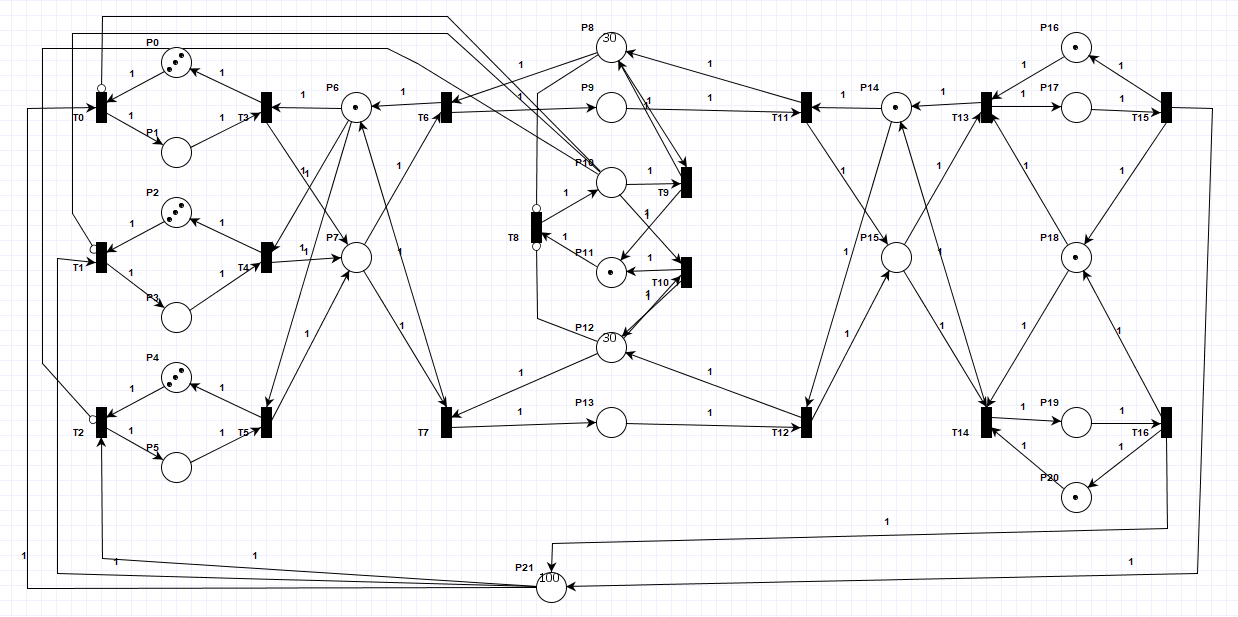
\includegraphics[width=0.75\textwidth]{RedDePetri}
		\caption{Red de Petri que modela el estacionamiento}
		\label{fig:mesh1}
	\end{figure}
	\subsection{Eventos y Estados}
	Las siguientes tablas tienen como objetivo exponer el significado fisico de las transiciones y plazas en la red de petri.
	\begin{table}[H]
		\begin{center}
		\begin{tabular}{ |c|c| } 
 			\hline
 			Transiciones & Eventos \\ 
 			T1 & Auto ingresa por calle 1 \\
 			T2 & Auto ingresa por calle 2 \\
 			T3 & Auto ingresa por calle 3 \\
 			T4 & Auto pasa barrera 1 \\
 			T5 & Auto pasa barrera 2 \\
 			T6 & Auto pasa barrera 3 \\ 
 			T7 & Auto ingresa al primer piso \\
 			T8 & Auto ingresa al segundo piso \\
 			T9 & Encender cartel \\
 			T10 & Apagar cartel por espacio disponible en piso 1 \\
 			T11 & Apagar cartel por espacio disponible en piso 2 \\
 			T12 & Auto sale del primer piso \\
 			T13 & Auto sale del segundo piso \\
 			T14 & Auto entrando a caja calle 1 \\
 			T15 & Auto entrando a caja calle 2 \\
 			T16 & Auto saliendo calle 1\\
 			T17 & Auto saliendo calle 2 \\ 
 			\hline
		\end{tabular}
		\end{center}
		\caption{Tabla de eventos.}
		\label{table:eventos}
	\end{table}
	
	\begin{table}[H]
		\begin{center}
		\begin{tabular}{ |c|c| } 
 			\hline
 			Plazas & Estados \\ 
 			P1 & Espacios disponibles de espera antes de la barrera 1 \\
 			P2 & Autos esperando antes de la barrera 1 \\
 			P3 & Espacios disponibles de espera antes de la barrera 2 \\
 			P4 & Autos esperando antes de la barrera 2 \\
 			P5 & Espacios disponibles de espera antes de la barrera 3 \\
 			P6 & Autos esperando antes de la barrera 3 \\ 
 			P7 & Lugar disponible en la calle de entrada \\
 			P8 & Auto circulando por la calle de entrada \\
 			P9 & Lugares disponibles para estacionar en el primer piso \\
 			P10 & Autos estacionados en el primer piso \\
 			P11 & Cartel encendido, es decir no hay lugar \\
 			P12 & Cartel apagado, es decir hay lugar \\
 			P13 & Lugares disponibles para estacionar en el segundo piso \\
 			P14 & Autos estacionados en el segundo piso \\
 			P15 & Lugar disponible en la calle de salida \\
 			P16 & Auto circulando por la calle de salida\\
 			P17 & Calle de salida 1\\
 			P18 & Auto pagando en la calle de salida 1 \\
 			P19 & Cajero/caja \\ 
 			P20 & Auto pagando en la calle de salida 2 \\
 			P21 &  Calle de salida 2\\
 			P22 & Autos totales \\
 			\hline
		\end{tabular}
		\end{center}
		\caption{Tabla de estados.}
		\label{table:estados}
	\end{table}
	\subsection{Analisis De La Red De Petri}
	Al realizar un analisis sobre la red de petri se pueden determinar las siguientes propiedades:
	\begin{itemize}
		\item Vivacidad: Al realizar el analisis concluimos que todas las transiciones 
		de la red pueden ser disparadas siempre y las que no pueden se verifica que 
		existe una secuencia de disparos que llevan a su sensibilizacion y posterior 
		disparo, por lo tanto se puede afirmar que la red tiene Vivacidad.
		\item Seguridad: La condición para que una Red de Petri sea segura es que cada 
		plaza que la compone debe tener como maximo un token. Por lo tanto esta red no es segura.
		\item Limitación: Una Red de Petri está limitada si todos las plazas están limitados por 
		un numero natural k, es decir que todas las plazas pueden contener a lo sumo k-token. 
		Por lo tanto la red es limitada.
		\item Libre de conflicto y conflictos estructurales: Se dice que existe un conflicto 
		estructural cuando al menos dos transiciones tienen una plaza en común. Podemos 
		observar que esto se cumple dos veces en esta red, por lo que no es libre de conflictos 
		y tiene conflictos estructurales. Ambos conflictos quedan denotados como:
		$K = < P_{8}\left\lbrace T_{7},T_{8}\right\rbrace >$
		$K = < P_{16}\left\lbrace T_{14},T_{15}\right\rbrace >$.
		\item Libre elección: Una red es de libre elección cuando las transiciones 
		que participan en un conflicto tienen una sola plaza de entrada. Por lo 
		tanto se puede afirmar que no tiene libre elección.
		\item Simple: La red es simple ya que las transiciones solo se ven afectadas 
		por solo un conflicto.
		\item Pura: Una Red de Petri es pura cuando no posee ningun auto-loop. En esta 
		red se encuentran dos auto-loop, por lo tanto no es pura. Estos auto-loops se 
		deben a que se utilizaron para modelar los arcos lectores.
		\item Capacidad finita: Cuando las plazas de la red están limitadas a un número 
		máximo de tokens, se dice que tiene capacidad finita, en este caso las plazas 
		pueden contener infinitos token por lo que la red no es de capacidad finita.
		Pero esto solo es debido a que las capcidades fueron modeladas a traves de una red ordinaria.
		\item Red de Petri No-autónoma: Una RdP no-autónoma es aquella que está 
		sincronizada/temporizada. Por lo tanto es no-autónoma.
		\item Interbloqueo: Se dice que una red presenta interbloqueo si tiene deadlock, 
		es decir alguna marca alcanzable desde donde no se puede disparar ninguna otra 
		transición.Por lo tanto esta red está libre de interbloqueo.
		\item Persistencia: Se dice que una Red de Petri es persistente si para cada 
		transición se cumple que dicha transición sólo puede ser desensibilizada por 
		su propio disparo. Por lo tanto y al existir conflicto estructural, esta red 
		no es persistente.
		\item Conservación: Se dice que una Red de Petri cumple con esta propiedad si 
		los tokens que se generan y consumen en la red permanecen constantes. Por lo 
		tanto es conservativa.
	\end{itemize}
	\subsubsection{Hilos}
	Una vez terminado el diseño de la red se procede a determinar la cantidad de hilos, donde se establecio que cada hilo disparara una transicion quedando asi un total de 17 hilos.
	\subsection{Invariantes}
	Los invariantes permiten caracterizar propiedades de las marcas alcanzables
	y de las tansiciones inalterables, independientemente de la evolucion, a continuacion se analizaran los invariantes de plaza y transicion.
		\subsubsection{Invariantes de Plaza}
		Un invariante de plaza es un subconjunto de lugares $P=\left\lbrace P_1,P_2,...,P_n \right\rbrace$ y un vector de ponderacion $\left\lbrace q_1,q_2,..., q_n \right\rbrace$ para el cual todos los pesos $q_i$ son enteros positivos tales que cumplen con:\newline
		$q_1*m(P_1),q_2*m(P_2),..., q_n*m(P_n)=K$ (constante) para cada $m\in M(m_0)$.\newline 
		Al analizar la red obtenemos los siguientes p-invariantes:
		\begin{itemize}
		\item $M(P0)+M(P1)=3$
		\item $M(P2)+M(P3)=3$
		\item $M(P4)+M(P5)=3$
		\item $M(P6)+M(P7)=1$
		\item $M(P8)+M(P9)=30$
		\item $M(P12)+M(P13)=30$
		\item $M(P14)+M(P15)=1$
		\item $M(P16)+M(P17)=1$
		\item $M(P19)+M(P20)=1$
		\item $M(P17)+M(P18)+M(P19)=1$
		\item $M(P1)+M(P3)+M(P5)+M(P7)+M(P9)+M(P13)+M(P15)+M(P17)+M(P19)+M(P21)=100$
		\item $M(P10)+M(P11)=1$
		\end{itemize}		
		\subsubsection{Invariantes de Transicion}
		Un invariante de transicion es aquella secuencia de transiciones disparadas tal que el estado de marcado final es igual al inicial. Al analizar la red obtenemos los siguientes t-invariantes:
		\begin{itemize}
		\item $\left\lbrace T0,T3,T6,TB,TD,TF \right\rbrace$
		\item $\left\lbrace T0,T3,T6,TB,TE,TX \right\rbrace$
		\item $\left\lbrace T0,T3,T7,TC,TD,TF \right\rbrace$
		\item $\left\lbrace T0,T3,T7,TC,TE,TX \right\rbrace$
		\item $\left\lbrace T1,T4,T6,TB,TD,TF \right\rbrace$
		\item $\left\lbrace T1,T4,T6,TB,TE,TX \right\rbrace$
		\item $\left\lbrace T1,T4,T7,TC,TD,TF \right\rbrace$
		\item $\left\lbrace T1,T4,T7,TC,TE,TX \right\rbrace$
		\item $\left\lbrace T2,T5,T6,TB,TD,TF \right\rbrace$
		\item $\left\lbrace T2,T5,T6,TB,TE,TX \right\rbrace$
		\item $\left\lbrace T2,T5,T7,TC,TD,TF \right\rbrace$
		\item $\left\lbrace T2,T5,T7,TC,TE,TX \right\rbrace$
		\item $\left\lbrace T8,T9 \right\rbrace$
		\item $\left\lbrace T8,TA \right\rbrace$
		\end{itemize}
	\subsection{Sistema Monitor Usando Programacion Orientada a Objetos}
	A continuacion mediante el uso de diagrams UML se describira como esta estructurado el sistema.
		\subsubsection{Diagrama De Clases}
		En la figura \ref{fig:mesh2} observamos el diagrama de clases del sistema.
		\begin{figure}[H]
			\centering
			\includegraphics[width=0.75\textwidth]{Diagrama_de_Clase}
			\caption{Diagrama de clases del sistema.}
			\label{fig:mesh2}
		\end{figure}
		\subsubsection{Diagrama De Secuencia}
		A continuacion en la figura \ref{fig:mesh3} se presenta el diagrama de secuencia del sistema.
		\begin{figure}[H]
			\centering
			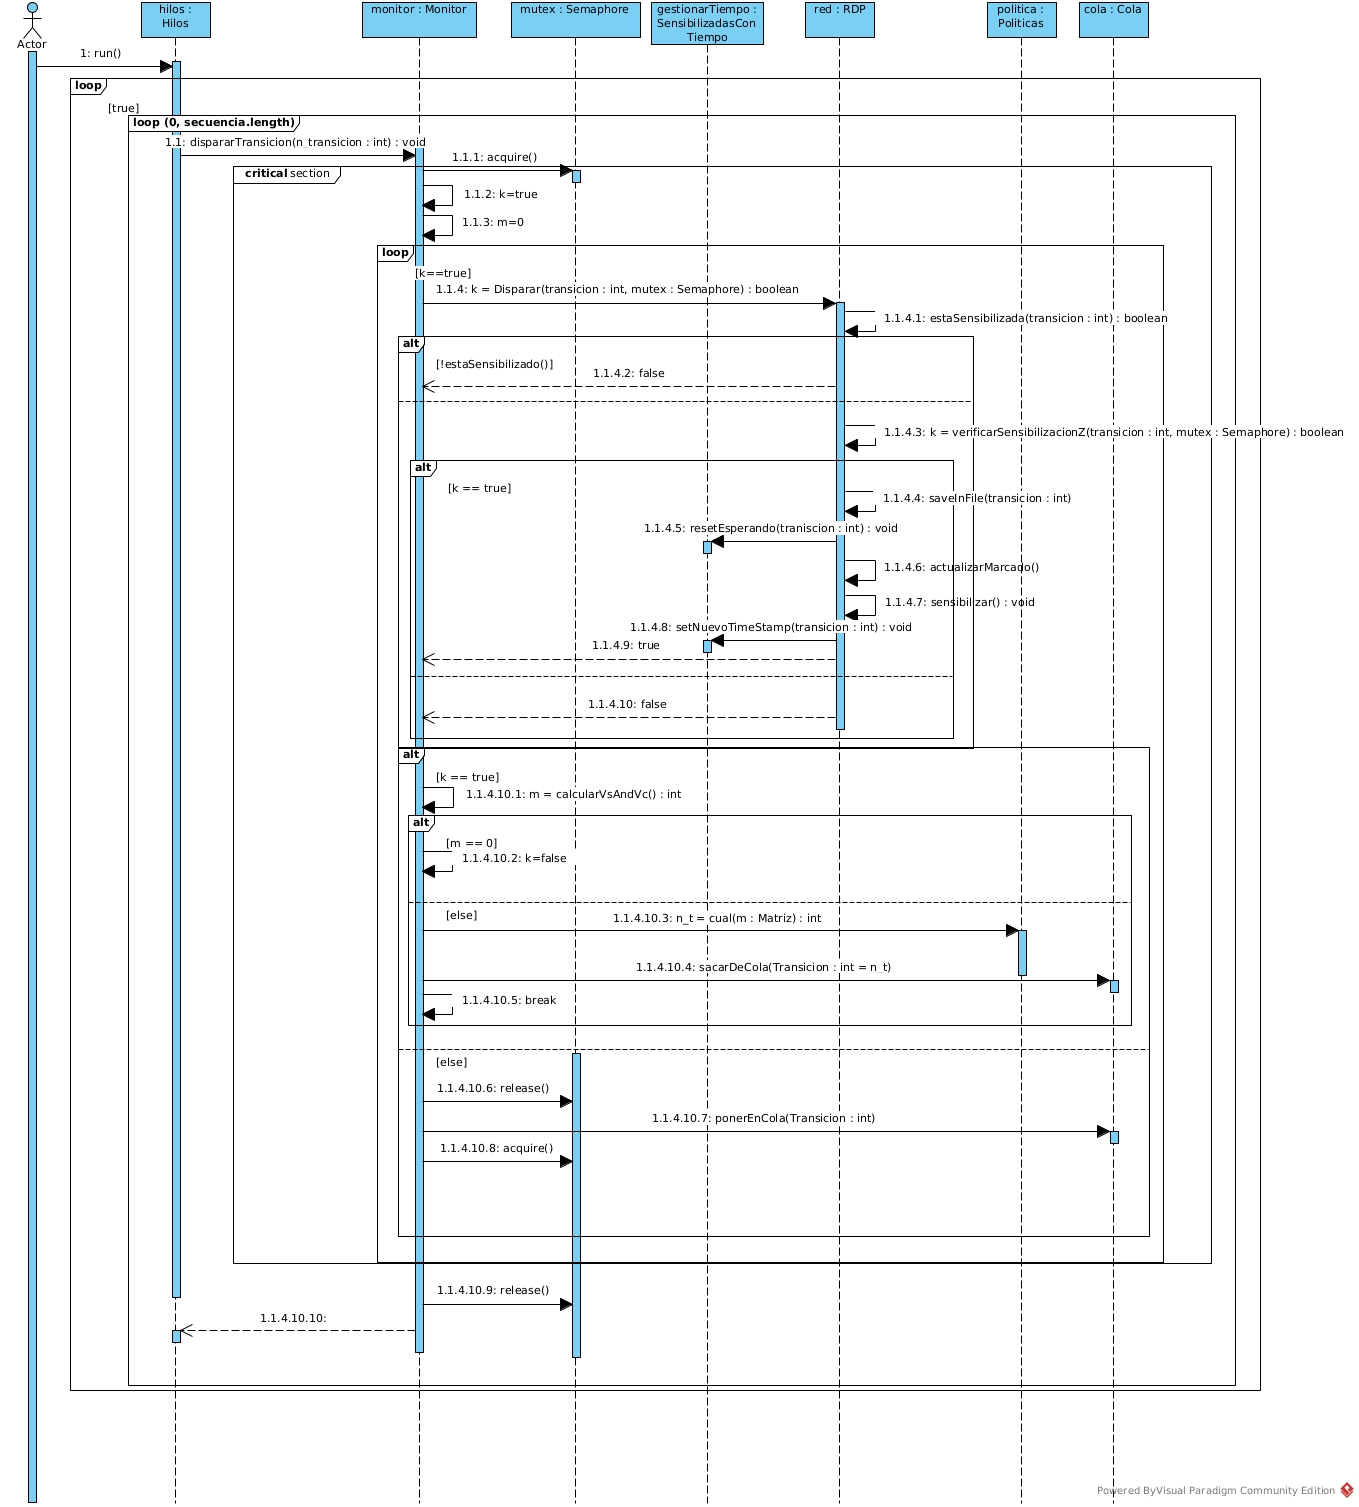
\includegraphics[width=0.75\textwidth]{Diagrama_de_secuencia}
			\caption{Diagrama de secuencia del sistema.}
			\label{fig:mesh3}
		\end{figure}
		\subsubsection{Verificacion De Invariantes}
		\textbf{P-Invariantes} \newline
		Para asegurar que los invariantes de plaza se cumplen se deben verificar las 
		expresiones anteriores cada vez que se realiza un disparo en la red, ya que 
		cada vez que lo hace se actualiza el marcado, en caso de no cumplirse el programa
		se detendra a traves del lanzamiento de una excepcion.\newline
		\textbf{T-Invariantes} \newline
		Para verificar los invariantes de transicion hay que ejecutar la simulacion una vez, 
		para luego a partir del archivo resultante extraer y armar las secuencias de disparo.
		Las secuencias se verifican a traves de un script python y mediante la libreria re el cual nos da acceso a las expresiones regulares. Lo primero es armar el patron para esto se uso una herramienta online llamada debuggex, en la figura \ref{fig:mesh4} observamos el resultado obtenido en la misma.		 
		\begin{figure}[H]
			\centering
			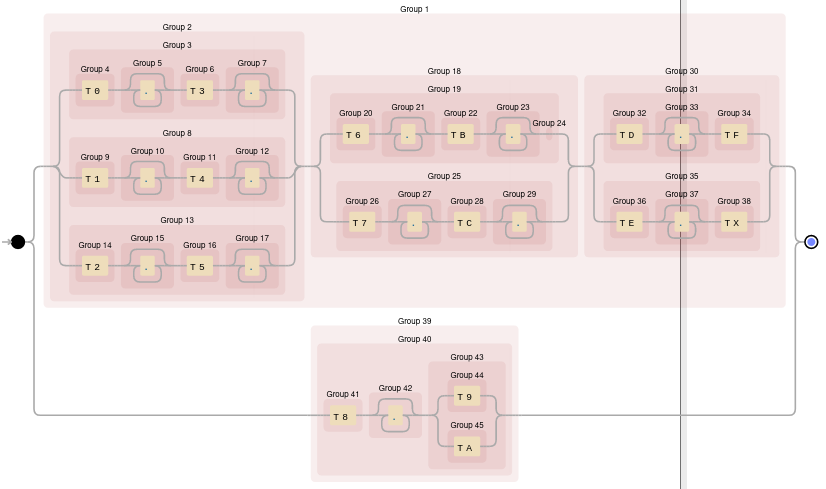
\includegraphics[width=0.75\textwidth]{debuggex}
			\caption{Diagrama del patron.}
			\label{fig:mesh4}
		\end{figure}

\section{Conclusion}
	Tras la finalización del presente trabajo se puede llegar a las siguientes conclusiones.
	Se aprendió las ventajas y desventajas de la programación concurrente. Algunas ventajas son la veloz ejecucion y tiempo de respuesta en un entorno multihilos, otra ventaja es la mejor utilizacion de las capacidades de los procesadore modernos. Algunas de las desventajas son la dificultad de debuggeo, ya que en un principio se presentaron problemas de exclusion mutua que no se cumplian al ingresar al recurso compartido.\newline
	Tambien se puede destacar las ventajas de realizar simulaciones con Redes de Petri, siendo las principales:
	\begin{itemize}
		\item El respaldo matematico que nos provee ya que esta nos brinda capacidad de validación 
		contra anomalias como son los bloqueos y fallas en la exclucion mutua.
		\item Facilidad para modelar las características relevantes de los sistemas concurrente (Concurrencia, 
		sincronización, bloqueos, etc.)
		\item Análisis y animación mediante simuladores basados en evento discretos.
	\end{itemize}
	
\section{Bibliografia}
	\begin{itemize}
		\item Ecuación de estado generalizada para redes de Petri no autónomas y con distintos tipos de arcos. Dr. Ing. Orlando Micolini1, Geol. Marcelo Cebollada y Verdaguer, Ing. Maximiliano Eschoyez, Ing. Luis Orlando Ventre, Ing. Marcelo Ismael Schild. Laboratorio de Arquitectura de Computadoras (LAC) FCEFyN Universidad Nacional de Córdoba.
		\item \url{https://www.debuggex.com/}.
		\item \href {https://docs.python.org/3/library/re.html}{https://docs.python.org/3/library/re.html}
	\end{itemize}
\end{document}
